% !TEX program = pdflatex
% !TEX options = -synctex=1 -interaction=nonstopmode -file-line-error "%DOC%"
% 作业模板
\documentclass[UTF8,10pt,a4paper]{article}
\usepackage{ctex}
\newfontfamily\menlo{MONACO.TTF}
\usepackage{amsmath}
\usepackage{diagbox}
\usepackage{float}
\usepackage{listings}
\usepackage{multirow}
\usepackage{tabularx}

\usepackage{url}
\usepackage{xcolor}
\newcommand{\tabincell}[2]{\begin{tabular}{@{}#1@{}}#2\end{tabular}}

\lstset{
    breaklines,                                 % 自动将长的代码行换行排版
    extendedchars=false,                        % 解决代码跨页时,章节标题,页眉等汉字不显示的问题
    backgroundcolor=\color[rgb]{0.96,0.96,0.96},% 背景颜色
    keywordstyle=\color{blue}\bfseries,         % 关键字颜色
    identifierstyle=\color{black},              % 普通标识符颜色
    commentstyle=\color[rgb]{0,0.6,0},          % 注释颜色
    stringstyle=\color[rgb]{0.58,0,0.82},       % 字符串颜色
    showstringspaces=false,                     % 不显示字符串内的空格
    numbers=left,                               % 显示行号
    numberstyle=\tiny\menlo,                    % 设置数字字体
    basicstyle=\small\menlo,                    % 设置基本字体
    captionpos=t,                               % title在上方(在bottom即为b)
    frame=single,                               % 设置代码框形式
    rulecolor=\color[rgb]{0.8,0.8,0.8},         % 设置代码框颜色
}  

\usepackage{pythonhighlight}
\usepackage{listings}
\usepackage{xcolor}
\usepackage{graphicx}
\usepackage[a4paper,left=2cm,right=2cm,top=2cm,bottom=2cm]{geometry}
\usepackage{fancyhdr}
% \catcode`\。=\active
% \newcommand{。}{.}
\newcommand{\CourseName}{操作系统(Operating System)}
\newcommand{\CourseCode}{CS307 \& CS356}
\newcommand{\Semester}{2020-2021学年第二学期}
\newcommand{\ProjectName} {\Huge{Project 4}} 
\newcommand{\StudentName}{刘涵之}
\newcommand{\StudentID}{519021910102}
\usepackage[vmargin=1in,hmargin=.5in]{geometry}
\usepackage{fancyhdr}
\usepackage{lastpage}
\usepackage{calc}
\pagestyle{fancy}
\fancyhf{}
\fancyhead[L]{\CourseName}
\fancyhead[C]{\ProjectName}
\fancyhead[R]{\StudentName}
\fancyfoot[R]{\thepage\ / \pageref{LastPage}}
\setlength\headheight{12pt}
\fancypagestyle{FirstPageStyle}{
    \fancyhf{}
    \fancyhead[L]{\CourseName\\
        \CourseCode\\
        \Semester}
    \fancyhead[C]{\large\bfseries\ProjectName \\}
    \fancyhead[R]{Name: \makebox[\widthof{\StudentID}][s]{\StudentName}\\
        ID : \StudentID\\
        }
    \fancyfoot[R]{\thepage\ / \pageref{LastPage}}
    \setlength\headheight{36pt}
}
\usepackage{amsmath,amssymb,amsthm,bm}
\allowdisplaybreaks[4]
\newtheoremstyle{Problem}
{}
{}
{}
{}
{\bfseries}
{.}
{ }
{第\thmnumber{ #2}\thmname{ #1}\thmnote{ (#3)} 得分: \underline{\qquad\qquad}}
\theoremstyle{Problem}
\newtheorem{prob}{题}
\newtheoremstyle{Solution}
{}
{}
{}
{}
{\bfseries}
{:}
{ }
{\thmname{#1}}
\makeatletter
\def\@endtheorem{\qed\endtrivlist\@endpefalse}
\makeatother
\theoremstyle{Solution}
\newtheorem*{sol}{解}
\title{Project 4: 
Scheduling Algorithms}
\date{}
% \usepackage{graphicx}
\begin{document}
\maketitle
\thispagestyle{FirstPageStyle}

This project involves implementing several different process scheduling algorithms. The scheduler will be assigned a predefined set of tasks and will schedule the tasks based on the selected scheduling algorithm. Each task is assigned a priority and CPU burst. The following scheduling algorithms will be implemented:

\begin{itemize}
    \item First-come, first-served (FCFS), which schedules tasks in the order in which they request the CPU.
    \item Shortest-job-first (SJF), which schedules tasks in order of the length of the tasks’ next CPU burst.
    \item Priority scheduling, which schedules tasks based on priority.
    \item Round-robin (RR) scheduling, where each task is run for a time quantum (or for the remainder of its CPU burst).
    \item Priority with round-robin, which schedules tasks in order of priority and uses round-robin scheduling for tasks with equal priority.
\end{itemize}

Priorities range from 1 to 10, where a higher numeric value indicates a higher relative priority. For round-robin scheduling, the length of a time quantum is 10 milliseconds.

The implementation of this project may be completed in either C or Java, and the program files supporting both of these languages are provided in the source code download for the textbook. These supporting files read in the schedule of tasks, insert the tasks into a list, and invoke the scheduler.

The schedule of tasks has the form \textbf{\textit{[task name] [priority] [CPU burst]}}.

There are a few different strategies for organizing the list of tasks. One approach is to place all tasks in a single unordered list, where the strategy for task selection depends on the scheduling algorithm. You are likely to find the functionality of a general list to be more suitable when completing this project.

\textbf{Further Challenges}: two additional challenges are presented for this project:
\begin{itemize}
\item Each task provided to the scheduler is assigned a unique task (\texttt{tid}). If a scheduler is running in a SMP environment where each CPU is separately running its own scheduler, there is a possible race condition on the variable that is used to assign task identifiers. Fix this race condition using an atomic integer.

On Linux and macOS systems, the \textbf{\_\_sync\_fetch\_and\_add()} function
can be used to atomically increment an integer value.

\item Calculate the average turnaround time, waiting time and response time for each of the scheduling algorithms.
\end{itemize}

\subsection{FCFS Scheduling Algorithm}

\textbf{Design}: My design for this task is shown as follows:

\begin{itemize}
    \item A new task will be insert in the head of the process list, so the next task to run is in the tail of the process list.
    \item I use \textbf{\_\_sync\_fetch\_and\_add()} function (atomic operation add) to solve the racing conditions. (\textbf{Further Challenges})
    \item I modified the \texttt{task.h} to calculate the average turnaround time, waiting time and response time for each of the scheduling algorithms. (\textbf{Further Challenges})
\end{itemize}


The code of \texttt{task.h} is shown as follows.
\begin{lstlisting}[language = c]
/**
 * Representation of a task in the system.
 */

#ifndef TASK_H
#define TASK_H

extern int tid_value;

typedef struct state {
    int arrival;
    int waiting;
    int response;
    int turnaround;
    int last_execute;
} State;

// representation of a task
typedef struct task {
    char *name;
    int tid;
    int priority;
    int burst;
    State state;
} Task;



#endif
\end{lstlisting}

The main code of this task is shown as follows.
\begin{lstlisting}[language = c]
#include "schedulers.h"

#include <stdio.h>
#include <stdlib.h>
#include <string.h>
#include "list.h"

#include "cpu.h"
#include "task.h"

struct node *head = NULL; 

int time = 0;

void add(char *name, int priority, int burst) {
    Task *t = (Task *) malloc (sizeof(Task));

	t -> name = (char *) malloc (sizeof(char) * (1 + strlen(name)));
	strcpy(t -> name, name);
	t -> tid = __sync_fetch_and_add(&tid_value, 1);
	t -> priority = priority;
	t -> burst = burst;

	State *state = &(t -> state);
	state -> arrival = time;
	state -> last_execute = time;
	state -> waiting = 0;
	state -> response = 0;
	state -> turnaround = 0;

	insert(&head, t);
}

void schedule() {
	int task_num = 0;
	int turnaround_total = 0;
	int waiting_total = 0;
	int response_total = 0;

	while(head != NULL) {
		struct node *h = head;
		while (h -> next != NULL) {
			h = h -> next;
		}

		Task *task = h -> task;
		run(task, task -> burst);
		delete(&head, task);

		State *state = &(task -> state);
		state -> waiting += time - state -> last_execute;
		if (state -> last_execute == state -> arrival) {
			state -> response = time - state -> last_execute;
		}
		state -> last_execute = time + task -> burst;
		state -> turnaround = time + task -> burst - state -> arrival;
		
		task_num ++;
		turnaround_total += state -> turnaround;
		waiting_total += state -> waiting;
		response_total += state -> response;

		time += task -> burst;

		free(task -> name);
		free(task);
	}
	printf("-----------------RESULT---------------------\n");
	printf("Total Time: %d , Total Task: %d \n", time, task_num);
	printf("Waiting Time: %d , Average: %.2lf \n", waiting_total, (double)waiting_total / task_num);
	printf("Turnaround Time: %d , Average: %.2lf \n", turnaround_total, (double)turnaround_total / task_num);
	printf("Response Time: %d , Average: %.2lf \n", response_total, (double)response_total / task_num);
	printf("-----------------RESULT---------------------\n");
}
\end{lstlisting}

The FCFS scheduler can be executed with the following instructions.
\begin{lstlisting}
make fcfs
./fcfs schedule.txt
\end{lstlisting}

The execution result of the program is shown as follow.

\begin{figure}[H]
    \centering
    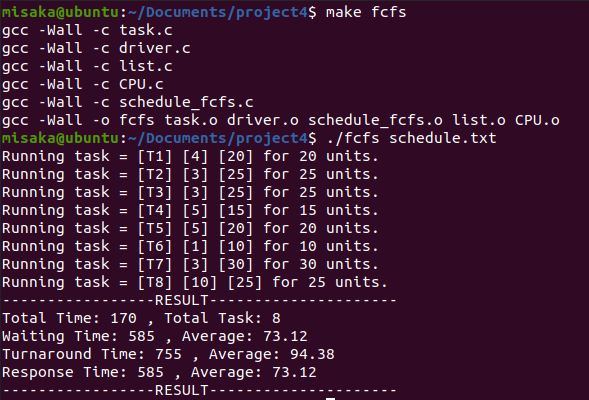
\includegraphics[width=400pt]{1fcfs.png}
    \caption{FCFS Scheduler}
    \label{3}
\end{figure}




\subsection{SJF Scheduling Algorithm}

\textbf{Design}: My design for this task is shown as follows:

\begin{itemize}
    \item The program need to find the process with the shortest burst time in the process list. I traverse the process list to find out the target process and execute it.
    \item \textbf{Further Challenges} are solved using the similar method as the first task.
\end{itemize}

The main code of this task is shown as follows.
\begin{lstlisting}[language = c]
#include "schedulers.h"

#include <stdio.h>
#include <stdlib.h>
#include <string.h>
#include "list.h"

#include "cpu.h"
#include "task.h"

struct node *head = NULL; 

int time = 0;

void add(char *name, int priority, int burst) {
    Task *t = (Task *) malloc (sizeof(Task));

	t -> name = (char *) malloc (sizeof(char) * (1 + strlen(name)));
	strcpy(t -> name, name);
	t -> tid = __sync_fetch_and_add(&tid_value, 1);
	t -> priority = priority;
	t -> burst = burst;

	State *state = &(t -> state);
	state -> arrival = time;
	state -> last_execute = time;
	state -> waiting = 0;
	state -> response = 0;
	state -> turnaround = 0;

	insert(&head, t);
}

void schedule() {
	int task_num = 0;
	int turnaround_total = 0;
	int waiting_total = 0;
	int response_total = 0;

	while(head != NULL) {
		struct node *h = head;
        struct node *i = head;
		while (i != NULL) {
			if (i -> task -> burst < h -> task -> burst) {
                h = i;
            }
            i = i -> next;
		}

		Task *task = h -> task;
		run(task, task -> burst);
		delete(&head, task);

		State *state = &(task -> state);
		state -> waiting += time - state -> last_execute;
		if (state -> last_execute == state -> arrival) {
			state -> response = time - state -> last_execute;
		}
		state -> last_execute = time + task -> burst;
		state -> turnaround = time + task -> burst - state -> arrival;
		
		task_num ++;
		turnaround_total += state -> turnaround;
		waiting_total += state -> waiting;
		response_total += state -> response;

		time += task -> burst;

		free(task -> name);
		free(task);
	}
	printf("-----------------RESULT---------------------\n");
	printf("Total Time: %d , Total Task: %d \n", time, task_num);
	printf("Waiting Time: %d , Average: %.2lf \n", waiting_total, (double)waiting_total / task_num);
	printf("Turnaround Time: %d , Average: %.2lf \n", turnaround_total, (double)turnaround_total / task_num);
	printf("Response Time: %d , Average: %.2lf \n", response_total, (double)response_total / task_num);
	printf("-----------------RESULT---------------------\n");
}
\end{lstlisting}

The SJF scheduler can be executed with the following instructions.
\begin{lstlisting}
make sjf
./sjf schedule.txt
\end{lstlisting}

The execution result of the program is shown as follow.

\begin{figure}[H]
    \centering
    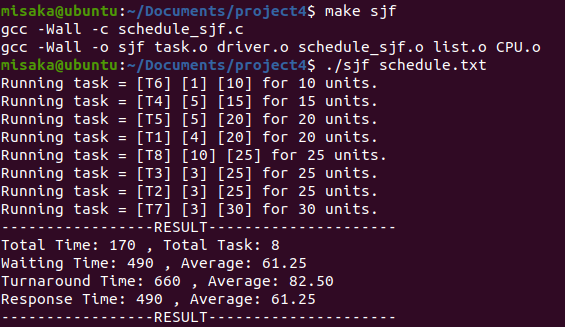
\includegraphics[width=400pt]{2sjf.png}
    \caption{SJF Scheduler}
\end{figure}

\subsection{Priority Scheduling Algorithm}

\textbf{Design}: My design for this task is shown as follows:

\begin{itemize}
    \item The program need to find the process with the highest priority in the process list. I traverse the process list to find out the target process and execute it.
    \item \textbf{Further Challenges} are solved using the similar method as the first task.
\end{itemize}

The main code of this task is shown as follows.
\begin{lstlisting}[language = c]
#include "schedulers.h"

#include <stdio.h>
#include <stdlib.h>
#include <string.h>
#include "list.h"

#include "cpu.h"
#include "task.h"

struct node *head = NULL; 

int time = 0;

void add(char *name, int priority, int burst) {
    Task *t = (Task *) malloc (sizeof(Task));

	t -> name = (char *) malloc (sizeof(char) * (1 + strlen(name)));
	strcpy(t -> name, name);
	t -> tid = __sync_fetch_and_add(&tid_value, 1);
	t -> priority = priority;
	t -> burst = burst;

	State *state = &(t -> state);
	state -> arrival = time;
	state -> last_execute = time;
	state -> waiting = 0;
	state -> response = 0;
	state -> turnaround = 0;

	insert(&head, t);
}

void schedule() {
	int task_num = 0;
	int turnaround_total = 0;
	int waiting_total = 0;
	int response_total = 0;

	while(head != NULL) {
		struct node *h = head;
        struct node *i = head;
		while (i != NULL) {
			if (i -> task -> priority >= h -> task -> priority) {
                h = i;
            }
            i = i -> next;
		}

		Task *task = h -> task;
		run(task, task -> burst);
		delete(&head, task);

		State *state = &(task -> state);
		state -> waiting += time - state -> last_execute;
		if (state -> last_execute == state -> arrival) {
			state -> response = time - state -> last_execute;
		}
		state -> last_execute = time + task -> burst;
		state -> turnaround = time + task -> burst - state -> arrival;
		
		task_num ++;
		turnaround_total += state -> turnaround;
		waiting_total += state -> waiting;
		response_total += state -> response;

		time += task -> burst;

		free(task -> name);
		free(task);
	}
	printf("-----------------RESULT---------------------\n");
	printf("Total Time: %d , Total Task: %d \n", time, task_num);
	printf("Waiting Time: %d , Average: %.2lf \n", waiting_total, (double)waiting_total / task_num);
	printf("Turnaround Time: %d , Average: %.2lf \n", turnaround_total, (double)turnaround_total / task_num);
	printf("Response Time: %d , Average: %.2lf \n", response_total, (double)response_total / task_num);
	printf("-----------------RESULT---------------------\n");
}
\end{lstlisting}

The priority scheduler can be executed with the following instructions.
\begin{lstlisting}
make Priority
./priority schedule.txt
\end{lstlisting}

The execution result of the program is shown as follow.

\begin{figure}[H]
    \centering
    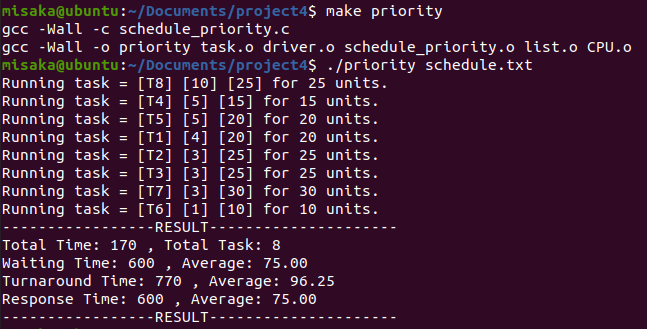
\includegraphics[width=400pt]{4pri.png}
    \caption{Priority Scheduler}
    \label{3}
\end{figure}

\subsection{RR Scheduling Algorithm}

\textbf{Design}: My design for this task is shown as follows:

\begin{itemize}
    \item The program need to execute the tasks in the task list one by one with a given execution time for each task.
    \item The current task is executed for a time slice, and if it is not finished, it will be put into the process list waiting for the next execution.
    \item \textbf{Further Challenges} are solved using the similar method as the first task.
\end{itemize}

The main code of this task is shown as follows.
\begin{lstlisting}[language = c]
#include "schedulers.h"

#include <stdio.h>
#include <stdlib.h>
#include <string.h>
#include "list.h"

#include "cpu.h"
#include "task.h"

struct node *head = NULL; 

int time = 0;

void add(char *name, int priority, int burst) {
    Task *t = (Task *) malloc (sizeof(Task));

	t -> name = (char *) malloc (sizeof(char) * (1 + strlen(name)));
	strcpy(t -> name, name);
	t -> tid = __sync_fetch_and_add(&tid_value, 1);
	t -> priority = priority;
	t -> burst = burst;

	State *state = &(t -> state);
	state -> arrival = time;
	state -> last_execute = time;
	state -> waiting = 0;
	state -> response = 0;
	state -> turnaround = 0;

	insert(&head, t);
}

void schedule() {
	int task_num = 0;
	int turnaround_total = 0;
	int waiting_total = 0;
	int response_total = 0;

	while(head != NULL) {
		struct node *h = head;
		while (h -> next != NULL) {
			h = h -> next;
		}

		Task *task = h -> task;

		if (task -> burst <= QUANTUM) {
			run(task, task -> burst);
			delete(&head, task);

			State *state = &(task -> state);
			state -> waiting += time - state -> last_execute;
			if (state -> last_execute == state -> arrival) {
				state -> response = time - state -> last_execute;
			}
			state -> last_execute = time + task -> burst;
			state -> turnaround = time + task -> burst - state -> arrival;
		
			task_num ++;
			turnaround_total += state -> turnaround;
			waiting_total += state -> waiting;
			response_total += state -> response;

			time += task -> burst;

			free(task -> name);
			free(task);
		} else {
			run(task, QUANTUM);
			delete(&head, task);
			task -> burst = task -> burst - QUANTUM;

			State *state = &(task -> state);
			state -> waiting += time - state -> last_execute;
			if (state -> last_execute == state -> arrival) {
				state -> response = time - state -> last_execute;
			}
			state -> last_execute = time + QUANTUM;

			time += QUANTUM;
			insert(&head, task);
		}

		
	}
	printf("-----------------RESULT---------------------\n");
	printf("Total Time: %d , Total Task: %d \n", time, task_num);
	printf("Waiting Time: %d , Average: %.2lf \n", waiting_total, (double)waiting_total / task_num);
	printf("Turnaround Time: %d , Average: %.2lf \n", turnaround_total, (double)turnaround_total / task_num);
	printf("Response Time: %d , Average: %.2lf \n", response_total, (double)response_total / task_num);
	printf("-----------------RESULT---------------------\n");
}
\end{lstlisting}

The RR scheduler can be executed with the following instructions.
\begin{lstlisting}
make rr
./rr schedule.txt
\end{lstlisting}

The execution result of the program is shown as follow.

\begin{figure}[H]
    \centering
    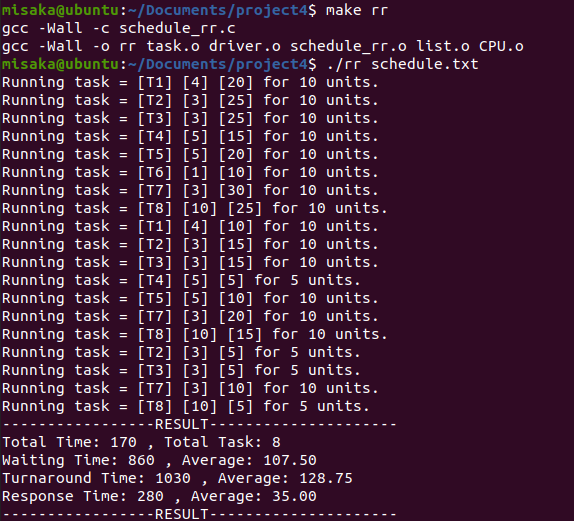
\includegraphics[width=400pt]{3rr.png}
    \caption{RR Scheduler}
    \label{3}
\end{figure}

\subsection{Priority-RR Scheduling Algorithm}

\textbf{Design}: My design for this task is shown as follows:

\begin{itemize}
    \item The program need to execute the tasks in the task list in order of priority with a given execution time for each task. 
    \item First, find the process(es) with the highest priority, and then use RR algorithm to execute them.
    \item The current process is executed for a time slice, and if it is not finished, it will be put into the process list waiting for the next execution.
    \item \textbf{Further Challenges} are solved using the similar method as the first task.
\end{itemize}

The main code of this task is shown as follows.
\begin{lstlisting}[language = c]
#include "schedulers.h"

#include <stdio.h>
#include <stdlib.h>
#include <string.h>
#include "list.h"

#include "cpu.h"
#include "task.h"

struct node *head = NULL; 

int time = 0;

void add(char *name, int priority, int burst) {
    Task *t = (Task *) malloc (sizeof(Task));

	t -> name = (char *) malloc (sizeof(char) * (1 + strlen(name)));
	strcpy(t -> name, name);
	t -> tid = __sync_fetch_and_add(&tid_value, 1);
	t -> priority = priority;
	t -> burst = burst;

	State *state = &(t -> state);
	state -> arrival = time;
	state -> last_execute = time;
	state -> waiting = 0;
	state -> response = 0;
	state -> turnaround = 0;

	insert(&head, t);
}

void schedule() {
	int task_num = 0;
	int turnaround_total = 0;
	int waiting_total = 0;
	int response_total = 0;

	while(head != NULL) {
		struct node *h = head;
        struct node *i = head;
		while (i != NULL) {
			if (i -> task -> priority >= h -> task -> priority) {
                h = i;
            }
            i = i -> next;
		}
        
		Task *task = h -> task;

		if (task -> burst <= QUANTUM) {
			run(task, task -> burst);
			delete(&head, task);

			State *state = &(task -> state);
			state -> waiting += time - state -> last_execute;
			if (state -> last_execute == state -> arrival) {
				state -> response = time - state -> last_execute;
			}
			state -> last_execute = time + task -> burst;
			state -> turnaround = time + task -> burst - state -> arrival;
		
			task_num ++;
			turnaround_total += state -> turnaround;
			waiting_total += state -> waiting;
			response_total += state -> response;

			time += task -> burst;

			free(task -> name);
			free(task);
		} else {
			run(task, QUANTUM);
			delete(&head, task);
			task -> burst = task -> burst - QUANTUM;

			State *state = &(task -> state);
			state -> waiting += time - state -> last_execute;
			if (state -> last_execute == state -> arrival) {
				state -> response = time - state -> last_execute;
			}
			state -> last_execute = time + QUANTUM;

			time += QUANTUM;
			insert(&head, task);
		}

		
	}
	printf("-----------------RESULT---------------------\n");
	printf("Total Time: %d , Total Task: %d \n", time, task_num);
	printf("Waiting Time: %d , Average: %.2lf \n", waiting_total, (double)waiting_total / task_num);
	printf("Turnaround Time: %d , Average: %.2lf \n", turnaround_total, (double)turnaround_total / task_num);
	printf("Response Time: %d , Average: %.2lf \n", response_total, (double)response_total / task_num);
	printf("-----------------RESULT---------------------\n");
}
\end{lstlisting}

The Priority-RR scheduler can be executed with the following instructions.
\begin{lstlisting}
make priority_rr
./priority_rr schedule.txt
\end{lstlisting}

The execution result of the program is shown as follow.

\begin{figure}[H]
    \centering
    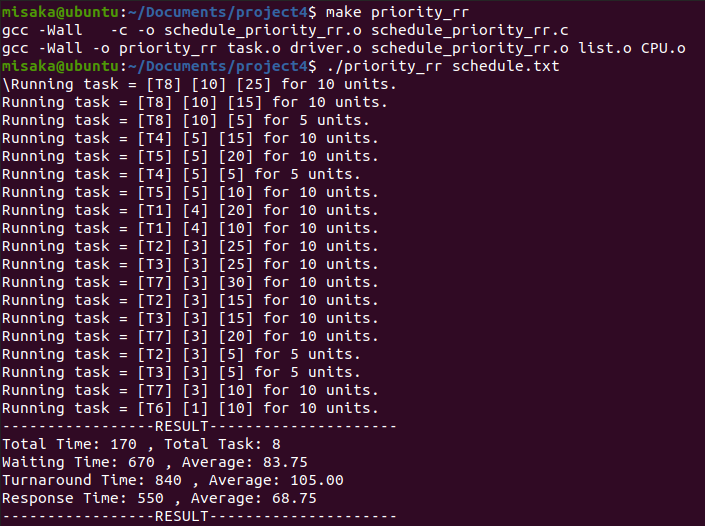
\includegraphics[width=400pt]{5prirr.png}
    \caption{Priority-RR Scheduler}
    \label{3}
\end{figure}


\end{document}